% !TeX root = ../thuthesis-example.tex
\chapter{数据集分析与对比}
\section{开源数据集}
UNSW-NB15 数据集是 2015 年澳大利亚网络安全中心使用 IXIA Perfect Storm
工具模拟网络环境流量而生成的一个数据集。相比于 KDD99 是一个更为新近的
数据集,因此更能代表真实的网络流量。UNSW-NB15 数据集中包括 100GB
的.pcap 格式的原始网络流量,同时还有 4 个经过特征提取的 csv 文件,分别是
UNSW-NB15\_1.csv  、 UNSW-NB15\_2.csv 、 UNSW-NB15\_3.csv  和   UNSW-
NB15\_4.csv,一共是 2540044 条数据,同时该数据集提出了与 KDD99 较为不同
的特征,这些特征更为符合当前的网络协议模式。 
UNSW-NB15 一共包含有 10 个分类,一个正常类别和 9 个攻击类别,其具体
描述和类别数目如下表所示: 
表 3.2 攻击类型描述和数目 

\begin{table}[]
    \begin{tabular}{lp{3cm}p{3cm}p{3cm}}
    \toprule
    类别      & 类别描述                                                                       & 样本数量    \\ \midrule
    Normal  & 正常流量                                                                       & 2218761 \\
    Fuzzers & 攻击者从命令行或以报文的形式发送大量随机生成的输入序列。攻击者试图发现操作系统、程序或网络中的安全漏洞,并使这些资源挂起一段时间,甚至可以使它们崩溃 & 24246   \\ \bottomrule
    \end{tabular}
    \end{table}

% \begin{table}[]
%     \centering
%     \begin{tabular}{lll}
%     % \begin{tabular}{@{}clllclcl@{}}
%     \toprule
%     类别 & 类别描述 & 样本数量 \\
%     % \multicolumn{4}{c}{类别}  & \multicolumn{2}{c}{类别描述} & \multicolumn{2}{c}{样本数量} \\
%     \midrule
%     Normal & 正常流量 & 2218761 \\
%     Fuzzers & 攻击者从命令行或以报文的形式发送大量随机生成的输入序列。攻击者试图发现操作系统、程序或网络中的安全漏洞,并使这些资源挂起一段时间,甚至可以使它们崩溃 & 24246 \\
%     % \multicolumn{4}{c}{Normal}  & \multicolumn{2}{c}{正常流量} & \multicolumn{2}{c}{2218761} \\
%     % \multicolumn{4}{c}{Fuzzers}  & \multicolumn{2}{c}{攻击者从命令行或以报文的形式发送大量随
%     % 机生成的输入序列。攻击者试图发现操作系
%     % 统、程序或网络中的安全漏洞,并使这些资
%     % 源挂起一段时间,甚至可以使它们崩溃。} & \multicolumn{2}{c}{24246} \\
%     \bottomrule
%     \end{tabular}
%     \end{table}

类别  类别描述  样本数量 
Normal  正常流量   
Fuzzers   
 
Analysis  这类攻击是指通过端口扫描、恶意 web 脚本
(如 HTML 文件渗透)和发送垃圾邮件等各种
方式渗透到 web 应用程序的各种入侵等。 
2677 
Backdoor  这类攻击中攻击者可以绕过正常的身份验证
并获得对系统的未授权远程访问。黑客利用
后门程序安装恶意文件,修改代码或获得对
系统或数据的访问。 
2329 
DoS  攻击者使某些计算或内存资源过于繁忙或占
据全部资源而无法处理合法请求或者拒绝合
法用户对计算机的访问。 
16353 

Exploit  利用操作系统或软件中的软件漏洞、漏洞或
故障进行入侵的行为。攻击者利用软件的知
识发动攻击,意图对系统造成危害。 
44525 

Generic  针对密码系统的攻击,试图破坏安全系统的
密钥。它独立于密码系统的实现细节。不考
虑块密码的结构。例如,生日攻击是一种将
哈希函数视为黑盒的通用攻击。 
215481 

Reconnaissance  为了绕过目标计算机网络的安全控制而收集
其信息的攻击。它可以被定义为一个探针,
是发起进一步攻击的初步步骤。攻击者使用
各种扫描手段来收集系统信息。在收集到足
够的信息后,可以发起后续的攻击。 
13987 

Shellcode  Shellcode 作为负载在目标机器执行,来挖掘
该软件的漏洞。之所以称作 Shellcode 是因为
启动了受到攻击者控制的命令行 shell。 
1511 

Worm  蠕虫是一种恶意程序或恶意软件,它可以复
制自己并传播到其他计算机。 
174 
 
UNSW-NB15 数据集一共包含 47 个特征,其中时间戳,IP 地址,端口号等特
征对训练无用,因此有效的特征一共 41 个。 
下面对这些特征做一个概括的说明。按照数据集作者的思路,可以分为基本
特征,内容特征,时间特征和额外生成的特征这几类。这里从另外一种思路进行
重新归类可以分为以下几类。


\begin{table}[]
    \begin{tabular}{|l|l|}
    \hline
    特征名称                  & 特征描述                      \\ \hline
    proto                 & 传输层协议                     \\ \hline
    service               & 应用层协议                     \\ \hline
    sttl                  & 从源发出的报文的 time to live     \\ \hline
    dttl                  & 从目的发出的报文的 time to live 字段 \\ \hline
    stcpb                 & 源 tcp 报文的初始序列号            \\ \hline
    dtcpb                 & 目的 tcp 报文的初始序列号           \\ \hline
    swin                  & 源 tcp 报文的窗口字段             \\ \hline
    dwin                  & 目的 tcp 报文的窗口字段            \\ \hline
    res\_bdy\_len         & http 响应内容的长度              \\ \hline
    ct\_flw\_http\_method & 会话中 http 方法字段的计数          \\ \hline
    is\_ftp\_login        & 是否有 ftp 的登录               \\ \hline
    ct\_ftp\_cmd          & 会话中 ftp 命令的计数             \\ \hline
    trans\_depth          & http 服务的连接深度              \\ \hline
    \end{tabular}
    \end{table}

表 3.4  与时间相关的特征 
\begin{table}[]
    \begin{tabular}{|l|l|}
    \hline
    dur     & 会话的持续时间                        \\ \hline
    tcprtt  & tcp 三次握手的 rtt(round trip time) \\ \hline
    synack  & 第一次发送到确认的时间                    \\ \hline
    ackdat  & 确认之后返回的时间                      \\ \hline
    sintpkt & 源报文的间隔时间的平均值                   \\ \hline
    dintpkt & 目的报文间隔时间的平均值                   \\ \hline
    sjit    & 源报文间隔时间的标准差(jitter)            \\ \hline
    djit    & 目的报文间隔时间的标准差                   \\ \hline
    sload   & 源报文的吞吐量                        \\ \hline
    dload   & 目的报文的吞吐量                       \\ \hline
    \end{tabular}
    \end{table}

    \begin{table}[]
        \begin{tabular}{|l|l|}
        \hline
        sbytes  & 会话中从源发出的总字节数  \\ \hline
        dbytes  & 会话中从目的发出的总字节数 \\ \hline
        smeansz & 会话中源报文的平均大小   \\ \hline
        dmeansz & 会话中目的报文的平均大小  \\ \hline
        spkts   & 会话中源的报文总数     \\ \hline
        dpkts   & 会话中目的报文总数     \\ \hline
        \end{tabular}
        \end{table}
表 3.6  与连接状态相关的特征 
\begin{table}[]
    \begin{tabular}{|l|l|}
    \hline
    sloss & 源的丢包数和重传数之和  \\ \hline
    dloss & 目的的丢包数和重传数之和 \\ \hline
    state & 会话的状态和相应的协议  \\ \hline
    \end{tabular}
    \end{table}
表 3.7  人工额外构造的特征 
\begin{table}[]
    \begin{tabular}{|l|l|}
    \hline
    ct\_srv\_src                & 根据最后一条报文的时间排序,每 100 条记录中源 \\ \hline
    ip 与服务都相同的会话计数(下面省略每 100 条) &                           \\ \hline
    ct\_srv\_dst                & 目的 IP 与服务都相同的会话计数         \\ \hline
    ct\_dst\_ltm                & 目的 IP 相同的会话计数             \\ \hline
    ct\_src\_ltm                & 源 IP 相同的会话计数              \\ \hline
    ct\_src\_dport\_ltm         & 源 IP 和目的端口都相同的会话计数        \\ \hline
    ct\_dst\_sport\_ltm         & 目的 IP 和源端口都相同的会话计数        \\ \hline
    ct\_dst\_src\_ltm           & 目的 IP 和源 IP 都相同的会话计数      \\ \hline
    ct\_state\_ttl              & 对于每一个状态,ttl 值的范围          \\ \hline
    is\_sm\_ips\_ports          & 源 ip 与目的 ip,源端口和目的端口是否都相同 \\ \hline
    \end{tabular}
    \end{table}
 
可以看到,UNSW-NB15 数据集大多数特征都有较为清晰的定义,因此可以
用做流量数据特征提取的标准。 
\section{校园网真实数据集预处理}

\chapter{基于图结构的RNN及其网络流量异常检测算法}

\section{引言}
Recurrent network的应用主要如下两部分:

文本相关。主要应用于自然语言处理(NLP)、对话系统、情感分析、机器翻译等等领域,Google翻译用的就是一个7-8层的LSTM模型。
时序相关。就是时序预测问题(timeseries),诸如预测天气、温度、包括个人认为根本不可行的但是很多人依旧在做的预测股票价格问题
这些问题都有一个共同点,就是有先后顺序的概念的。举个例子: 根据前5天每个小时的温度,来预测接下来1个小时的温度。典型的时序问题,温度是从5天前,一小时一小时的记录到现在的,它们的顺序不能改变,否则含义就发生了变化;再比如情感分析中,判断一个人写的一篇文章或者说的一句话,它是积极地(positive),还是消极的(negative),这个人说的话写的文章,里面每个字都是有顺序的,不能随意改变,否则含义就不同了。

全连接网络Fully-Connected Network,或者卷积神经网络Convnet,他们在处理一个sequence(比如一个人写的一条影评),或者一个timeseries of data points(比如连续1个月记录的温度)的时候,他们缺乏记忆。一条影评里的每一个字经过word embedding后,被当成了一个独立的个体输入到网络中;网络不清楚之前的,或者之后的文字是什么。这样的网络,我们称为feedforward network。

但是实际情况,我们理解一段文字的信息的时候,每个文字并不是独立的,我们的脑海里也有它的上下文。比如当你看到这段文字的时候,你还记得这篇文章开头表达过一些关于LSTM的信息;

所以,我们在脑海里维护一些信息,这些信息随着我们的阅读不断的更新,帮助我们来理解我们所看到的每一个字,每一句话。这就是RNN的做法:维护一些中间状态信息。
% \section{网络流量的时空特性}

% \section{基于图结构的RNN原理}
% 神经网络是目前计算机科学最流行的算法之一,它在图像识别、语音识别和自然语言处理等领域取得了重大突破。卷积神经网络、循环神经网络。
\section{神经网络}
神经网络(Neural Network,NN),又称人工神经网络(Artificial Neural Network,ANN),是20世纪80 年代以来人工智能领域兴起的研究热点。它的定义有很多,其中第一批神经计算机的发明者Robert Hecht-Nielsen博士对神经网络的定义是“ 一个由许多简单的,高度互连的处理元素组成的计算系统, 它们通过对外部输入的动态状态反应来处理信息。或者也可以认为人工神经网络是一种计算模型,它的灵感来自于人脑中生物神经网络处理信息的方式。”
最近十多年来,针对人工神经网络的研究工作已经取得了重大进展,其在模式识别、自动控制、预测估计等领域已成功地解决了许多现代计算机难以解决的实际问题。


神经网络的灵感来自于人脑生物神经网络的处理方式。
大脑的基本计算单位是神经元。在人类的神经系统中,大约有860亿个神经元,它们与大约$10^{14}$-$10^{15}$的突触相连。神经网络的基本计算单位也是神经元,通常称为节点或单位。它从其他一些节点或外部源接收输入,并计算输出。每个输入都有一个相关的权重(w),该权重是根据其对其他输入的相对重要性分配的。节点对其输入的加权和应用一个函数。
其想法是,突触强度(权重w)是可学习的,并控制影响的强度及其方向:一个神经元对另一个神经元的兴奋性(正权重)或抑制性(负权重)。在基本模型中,树突将信号传到细胞体,在那里它们都会被相加。如果最后的总和超过了某个阈值,神经元就可以开火,沿着轴突发出一个尖峰。在计算模型中,我们假设尖峰的精确时序并不重要,只有发射的频率能传递信息。我们用激活函数(e.x sigmoid函数)来模拟神经元的发射率,它代表沿轴突的尖峰频率。

从上面的解释我们可以得出结论,神经网络是由神经元组成的,生物学上神经元是通过突触连接的,信息在突触中流动(出计算模型的权重),当我们训练一个神经网络时,我们希望神经元每当从数据中学习到特定的模式时就开火,我们用激活函数来模拟开火率。

一个人工神经元的结构如图~\ref{fig:神经元}所示:
\begin{figure}
    \centering
    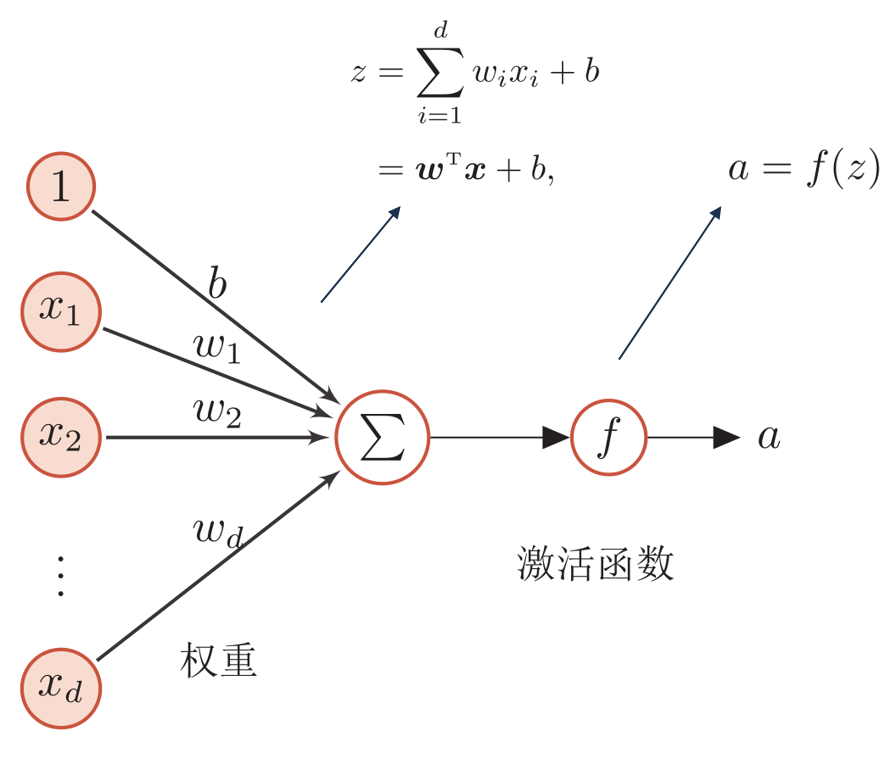
\includegraphics[width=0.6\linewidth]{人工神经元.png}
    \caption{人工神经元模型}
    \label{fig:神经元}
  \end{figure}

在图~\ref{fig:神经元}中,$\vec{x}$为输入向量,$w$和$b$分别是权重和偏移,

神经网络主要由以下几部分组成:
\begin{itemize}
    \item 输入节点(输入层)。在这一层中不进行任何计算,它们只是将信息传递给下一层(大部分时间是隐藏层)。一块节点也叫层。
    \item 隐藏节点(隐藏层)。在隐藏层中,中间处理或计算是在这里完成的,它们进行计算,然后将输入层的权重(信号或信息)传递给下一层(另一个隐藏层或输出层)。没有隐藏层的神经网络也是可以的,我后面会来解释这个问题。
    \item 输出节点(输出层):在这里,我们最后使用一个激活函数,映射到所需的输出格式(例如用于分类的softmax)。连接和权重。网络由连接组成,每个连接将神经元i的输出转移到神经元j的输入上,在这个意义上,i是j的前身,j是i的继任者,每个连接被赋予一个权重Wij。
    \item 激活函数:一个节点的激活函数定义了该节点给定输入或一组输入的输出。一个标准的计算机芯片电路可以看作是一个激活函数的数字网络,根据输入的不同,激活函数可以是 "ON"(1)或 "OFF"(0)。这与神经网络中线性感知器的行为类似。然而,正是由于非线性激活函数,使得这类网络只需使用少量的节点就能计算出非平凡的问题。在人工神经网络中,这个函数也被称为传递函数。
    \item 学习规则。学习规则是一种规则或算法,它修改神经网络的参数,以使网络的给定输入产生一个有利的输出。这个学习过程通常相当于修改权重和阈值。
\end{itemize}

神经网络有很多类型,这里本文将神经网络划分为前馈神经网络和循环神经网络,其中前馈神经网络包含单层感知机、多层感知机(MLP)、卷积神经网络(CNN)等。
本文主要介绍循环神经网络, 循环神经网络(Recurrent Neural Network,RNN)是一类具有短期记忆能力的神经网络。在循环神经网络中,神经元不但可以接受其他神经元的信息,也可以接受自身的信息,形成具有环路的网络结构.和前馈神经网络相比,循环神经网络更加符合生物神经网络的结构。
下图~\ref{fig:循环神经网络}是循环神经网络的示意图。
\begin{figure}
    \centering
    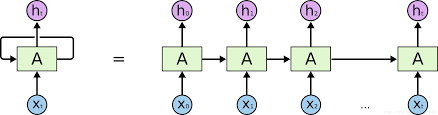
\includegraphics[width=0.6\linewidth]{循环神经网络.png}
    \caption{循环神经网络}
    \label{fig:循环神经网络}
  \end{figure}


神经网络的类型
神经网络有很多类,这些类也有子类,在这里我将列出最常用的类.
1. 前馈神经网络
前馈神经网络是一种人工神经网络,单元之间的连接不形成循环。在这种网络中,信息只有一个方向,即向前移动,从输入节点,通过隐藏节点(如果有的话),然后到输出节点。网络中不存在循环或环路。
我们可以区分两种类型的前馈神经网络。
1.1. 单层感知器
这是最简单的前馈神经网络,不包含任何隐藏层,也就是说它只由单层的输出节点组成。之所以说是单层,是因为我们在计算层数的时候,并不包括输入层,原因是在输入层没有进行计算,输入通过一系列的权重直接反馈给输出。

1.2. 多层感知器(MLP)
这类网络由多层计算单元组成,通常以前馈方式相互连接。一层中的每个神经元都与后一层的神经元有定向连接。在许多应用中,这些网络的单元应用一个sigmoid函数作为激活函数。MLP是非常有用的,一个很好的原因是,它们能够学习非线性表示(大多数情况下,呈现给我们的数据是不可线性分离的),我们会在下一篇文章中给大家展示的例子中再来分析这一点。

1.3. 卷积神经网络(CNN)
卷积神经网络与普通的神经网络非常相似,它们是由具有可学习权重和偏差的神经元组成的。在卷积神经网络(CNN,或ConvNet或移位不变或空间不变)中,单元连接模式的灵感来自于视觉皮层的组织,单元在一个被称为感受场的受限空间区域内对刺激做出反应。感受场部分重叠,覆盖了整个视场。单元响应可以用卷积运算在数学上近似。它们是多层感知器的变体,使用最少的预处理。它们的广泛应用是在图像和视频识别,推荐系统和自然语言处理。CNNs需要大量的数据来进行训练。

2. 循环神经网络
在循环神经网络(RNN)中,单元之间的连接形成了一个定向循环(它们向前传播数据,同时也向后传播数据,从较后的处理阶段到较早的阶段)。这使得它能够表现出动态的时间行为。与前馈神经网络不同,RNNs可以利用其内部存储器处理任意输入序列。这使得它们适用于未分割、连接的手写识别、语音识别和其他一般序列处理器等任务。

常用的激活功能
每一个激活函数(或者说非线性函数)都会取一个单数,并对其进行一定的固定数学运算。下面是一些常用的激活函数。
Sigmoid
sigmoid非线性的数学形式为σ(x)=1/(1+e-x),它将一个实值数 "压扁 "到0和1之间,特别是大的负数变成0,大的正数变成1。sigmoid函数在历史上被频繁使用,因为它有一个很好的解释,作为一个神经元的发射率:从完全不发射(0)到完全饱和的发射,在一个假设的最大频率(1)。在实践中,sigmoid非线性最近已经失宠,它很少被使用。它有两个主要的缺点。
Tanh
ReLU
Leaky ReLU

% 循环神经网络解决了这个问题。它们是带有循环的网络,允许信息持续存在。循环神经网络可以被认为是同一个网络的多个副本,每个副本都会向后继者传递信息。
\section{实验方案设计及实验流程}

\section{算法性能评估}

\subsection{基于开源数据集的检测结果}

\subsection{基于真实数据的检测结果}